\subsection{Recibir una actualización de partida}

\begin{figure}[ht]
\centering
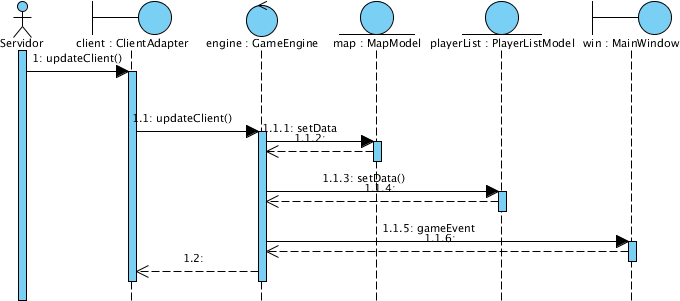
\includegraphics[scale=0.6]{img/ch03devel-update.png}
\caption{Diagrama de secuencia de ``Recibir una actualización de partida''}
\end{figure}

De manera asíncrona, y cada vez que otro jugador realice alguna acción sobre la
partida, el servidor enviará los datos que hayan cambiando para permanecer así
sincronizados con el resto de jugadores.

Estos datos son añadidos a los modelos de datos, los cuales actualizarán las
vistas que se encuentren observándolos.

Adicionalmente, se puede enviar un atributo que indique el tipo de evento. Si
tal es el caso, se llamará a la función correspondiente en la interfaz
\texttt{GameEventListener} que mostrará una mensaje en la ventana principal.
